%% Преамбула TeX-файла

% 1. Стиль и язык
\documentclass[utf8x, 12pt, twoside, a5paper]{G7-32} % Стиль (по умолчанию будет 14pt)

% Остальные стандартные настройки убраны в preamble-std.tex
\sloppy

% 1. Настройки стиля ГОСТ 7-32
% Для начала определяем, хотим мы или нет, чтобы рисунки и таблицы нумеровались в пределах раздела, или нам нужна сквозная нумерация.
% А не забыл ли автор букву 't' ?
\EqInChapter % формулы будут нумероваться в пределах раздела
\TableInChapter % таблицы будут нумероваться в пределах раздела
\PicInChapter % рисунки будут нумероваться в пределах раздела

% 2. Добавляем гипертекстовое оглавление в PDF
\usepackage[
bookmarks=true, colorlinks=true, unicode=true,
urlcolor=black,linkcolor=black, anchorcolor=black,
citecolor=black, menucolor=black, filecolor=black,
]{hyperref}

% 3. Изменение начертания шрифта --- после чего выглядит таймсоподобно.
% apt-get install scalable-cyrfonts-tex

\IfFileExists{cyrtimes.sty}
    {
        \usepackage{cyrtimespatched}
    }
    {
        % А если Times нету, то будет CM...
    }


% 4. Прочие полезные пакеты.
\usepackage{underscore} % Ура! Теперь можно писать подчёркивание.
                        % И нельзя использовать подчёркивание в файлах.
                        % Выбирай, но осторожно.

\usepackage{graphicx}   % Пакет для включения рисунков

 % 5. Любимые команды
\newcommand{\Code}[1]{\textbf{#1}}

% 6. Поля
% С такими оно полями оно работает по-умолчанию:
% \RequirePackage[left=20mm,right=10mm,top=20mm,bottom=20mm,headsep=0pt]{geometry}
% Если вас тошнит от поля в 10мм --- увеличивайте до 20-ти, ну и про переплёт не забывайте:


% Размер страницы
\usepackage{geometry}
%\geometry{paperheight=20cm}
%\geometry{paperwidth=15cm}

\geometry{right=20mm}
\geometry{left=20mm}
\geometry{top=8mm}
\geometry{bottom=15mm}

% 7. Tikz
\usepackage{tikz}
\usetikzlibrary{arrows,positioning,shadows}

% 8 Листинги

\usepackage{listings}

% Значения по умолчанию
\lstset{
  basicstyle= \footnotesize,
  breakatwhitespace=true,% разрыв строк только на whitespacce
  breaklines=true,       % переносить длинные строки
%   captionpos=b,          % подписи снизу -- вроде не надо
  inputencoding=koi8-r,
  numbers=left,          % нумерация слева
  numberstyle=\footnotesize,
  showspaces=false,      % показывать пробелы подчеркиваниями -- идиотизм 70-х годов
  showstringspaces=false,
  showtabs=false,        % и табы тоже
  stepnumber=1,
  tabsize=4,              % кому нужны табы по 8 символов?
  frame=single
}

% Стиль для псевдокода: строчки обычно короткие, поэтому размер шрифта побольше
\lstdefinestyle{pseudocode}{
  basicstyle=\small,
  keywordstyle=\color{black}\bfseries\underbar,
  language=Pseudocode,
  numberstyle=\footnotesize,
  commentstyle=\footnotesize\it
}

% Стиль для обычного кода: маленький шрифт
\lstdefinestyle{realcode}{
  basicstyle=\scriptsize,
  numberstyle=\footnotesize
}

% Стиль для коротких кусков обычного кода: средний шрифт
\lstdefinestyle{simplecode}{
  basicstyle=\footnotesize,
  numberstyle=\footnotesize
}

% Стиль для BNF
\lstdefinestyle{grammar}{
  basicstyle=\footnotesize,
  numberstyle=\footnotesize,
  stringstyle=\bfseries\ttfamily,
  language=BNF
}

% Определим свой язык для написания псевдокодов на основе Python
\lstdefinelanguage[]{Pseudocode}[]{Python}{
  morekeywords={each,empty,wait,do},% ключевые слова добавлять сюда
  morecomment=[s]{\{}{\}},% комменты {а-ля Pascal} смотрятся нагляднее
  literate=% а сюда добавлять операторы, которые хотите отображать как мат. символы
    {->}{\ensuremath{$\rightarrow$}~}2%
    {<-}{\ensuremath{$\leftarrow$}~}2%
    {:=}{\ensuremath{$\leftarrow$}~}2%
    {<--}{\ensuremath{$\Longleftarrow$}~}2%
}[keywords,comments]

% Свой язык для задания грамматик в BNF
\lstdefinelanguage[]{BNF}[]{}{
  morekeywords={},
  morecomment=[s]{@}{@},
  morestring=[b]",%
  literate=%
    {->}{\ensuremath{$\rightarrow$}~}2%
    {*}{\ensuremath{$^*$}~}2%
    {+}{\ensuremath{$^+$}~}2%
    {|}{\ensuremath{$|$}~}2%
}[keywords,comments,strings]

% Подписи к листингам на русском языке.
\renewcommand*\thelstnumber{\oldstylenums{\the\value{lstnumber}}}
\renewcommand\lstlistingname{\cyr\CYRL\cyri\cyrs\cyrt\cyri\cyrn\cyrg}
\renewcommand\lstlistlistingname{\cyr\CYRL\cyri\cyrs\cyrt\cyri\cyrn\cyrg\cyri}

% Произвольная нумерация списков.
\usepackage{enumerate}

% Вставлять pdf-страницы
\usepackage{pdfpages}

\usepackage{fancyhdr}

\usepackage{multicol}


\raggedbottom
\captionsetup[figure]{belowskip=0pt,aboveskip=0pt}
\setlength{\intextsep}{3pt plus 0pt minus 0pt}

%\usepackage{sidecap}
%\usepackage{floatrow}

\usepackage{setspace}



%\usepackage[perpage,para,symbol*]{footmisc}

\usepackage{floatrow}

\begin{document}


\makeatletter
%\renewcommand{\@oddhead}{\hfill\thepage\hfill}
\renewcommand{\@oddfoot}{\hfill\thepage}
\renewcommand{\@evenfoot}{\thepage\hfill}

\makeatother

\frontmatter % выключает нумерацию ВСЕГО; здесь начинаются ненумерованные главы: реферат, введение, глоссарий, сокращения и прочее

% Команды \breakingbeforechapters и \nonbreakingbeforechapters
% управляют разрывом страницы перед главами.
% По-умолчанию страница разрывается.

% \nobreakingbeforechapters
% \breakingbeforechapters

\thispagestyle{empty} 

\begin{center}
М. В. Миникс

\vfill

\large Дворовые компании \\(о людях дома у Красных ворот)

\vfill

\begin{figure}[ht]
  \centering
  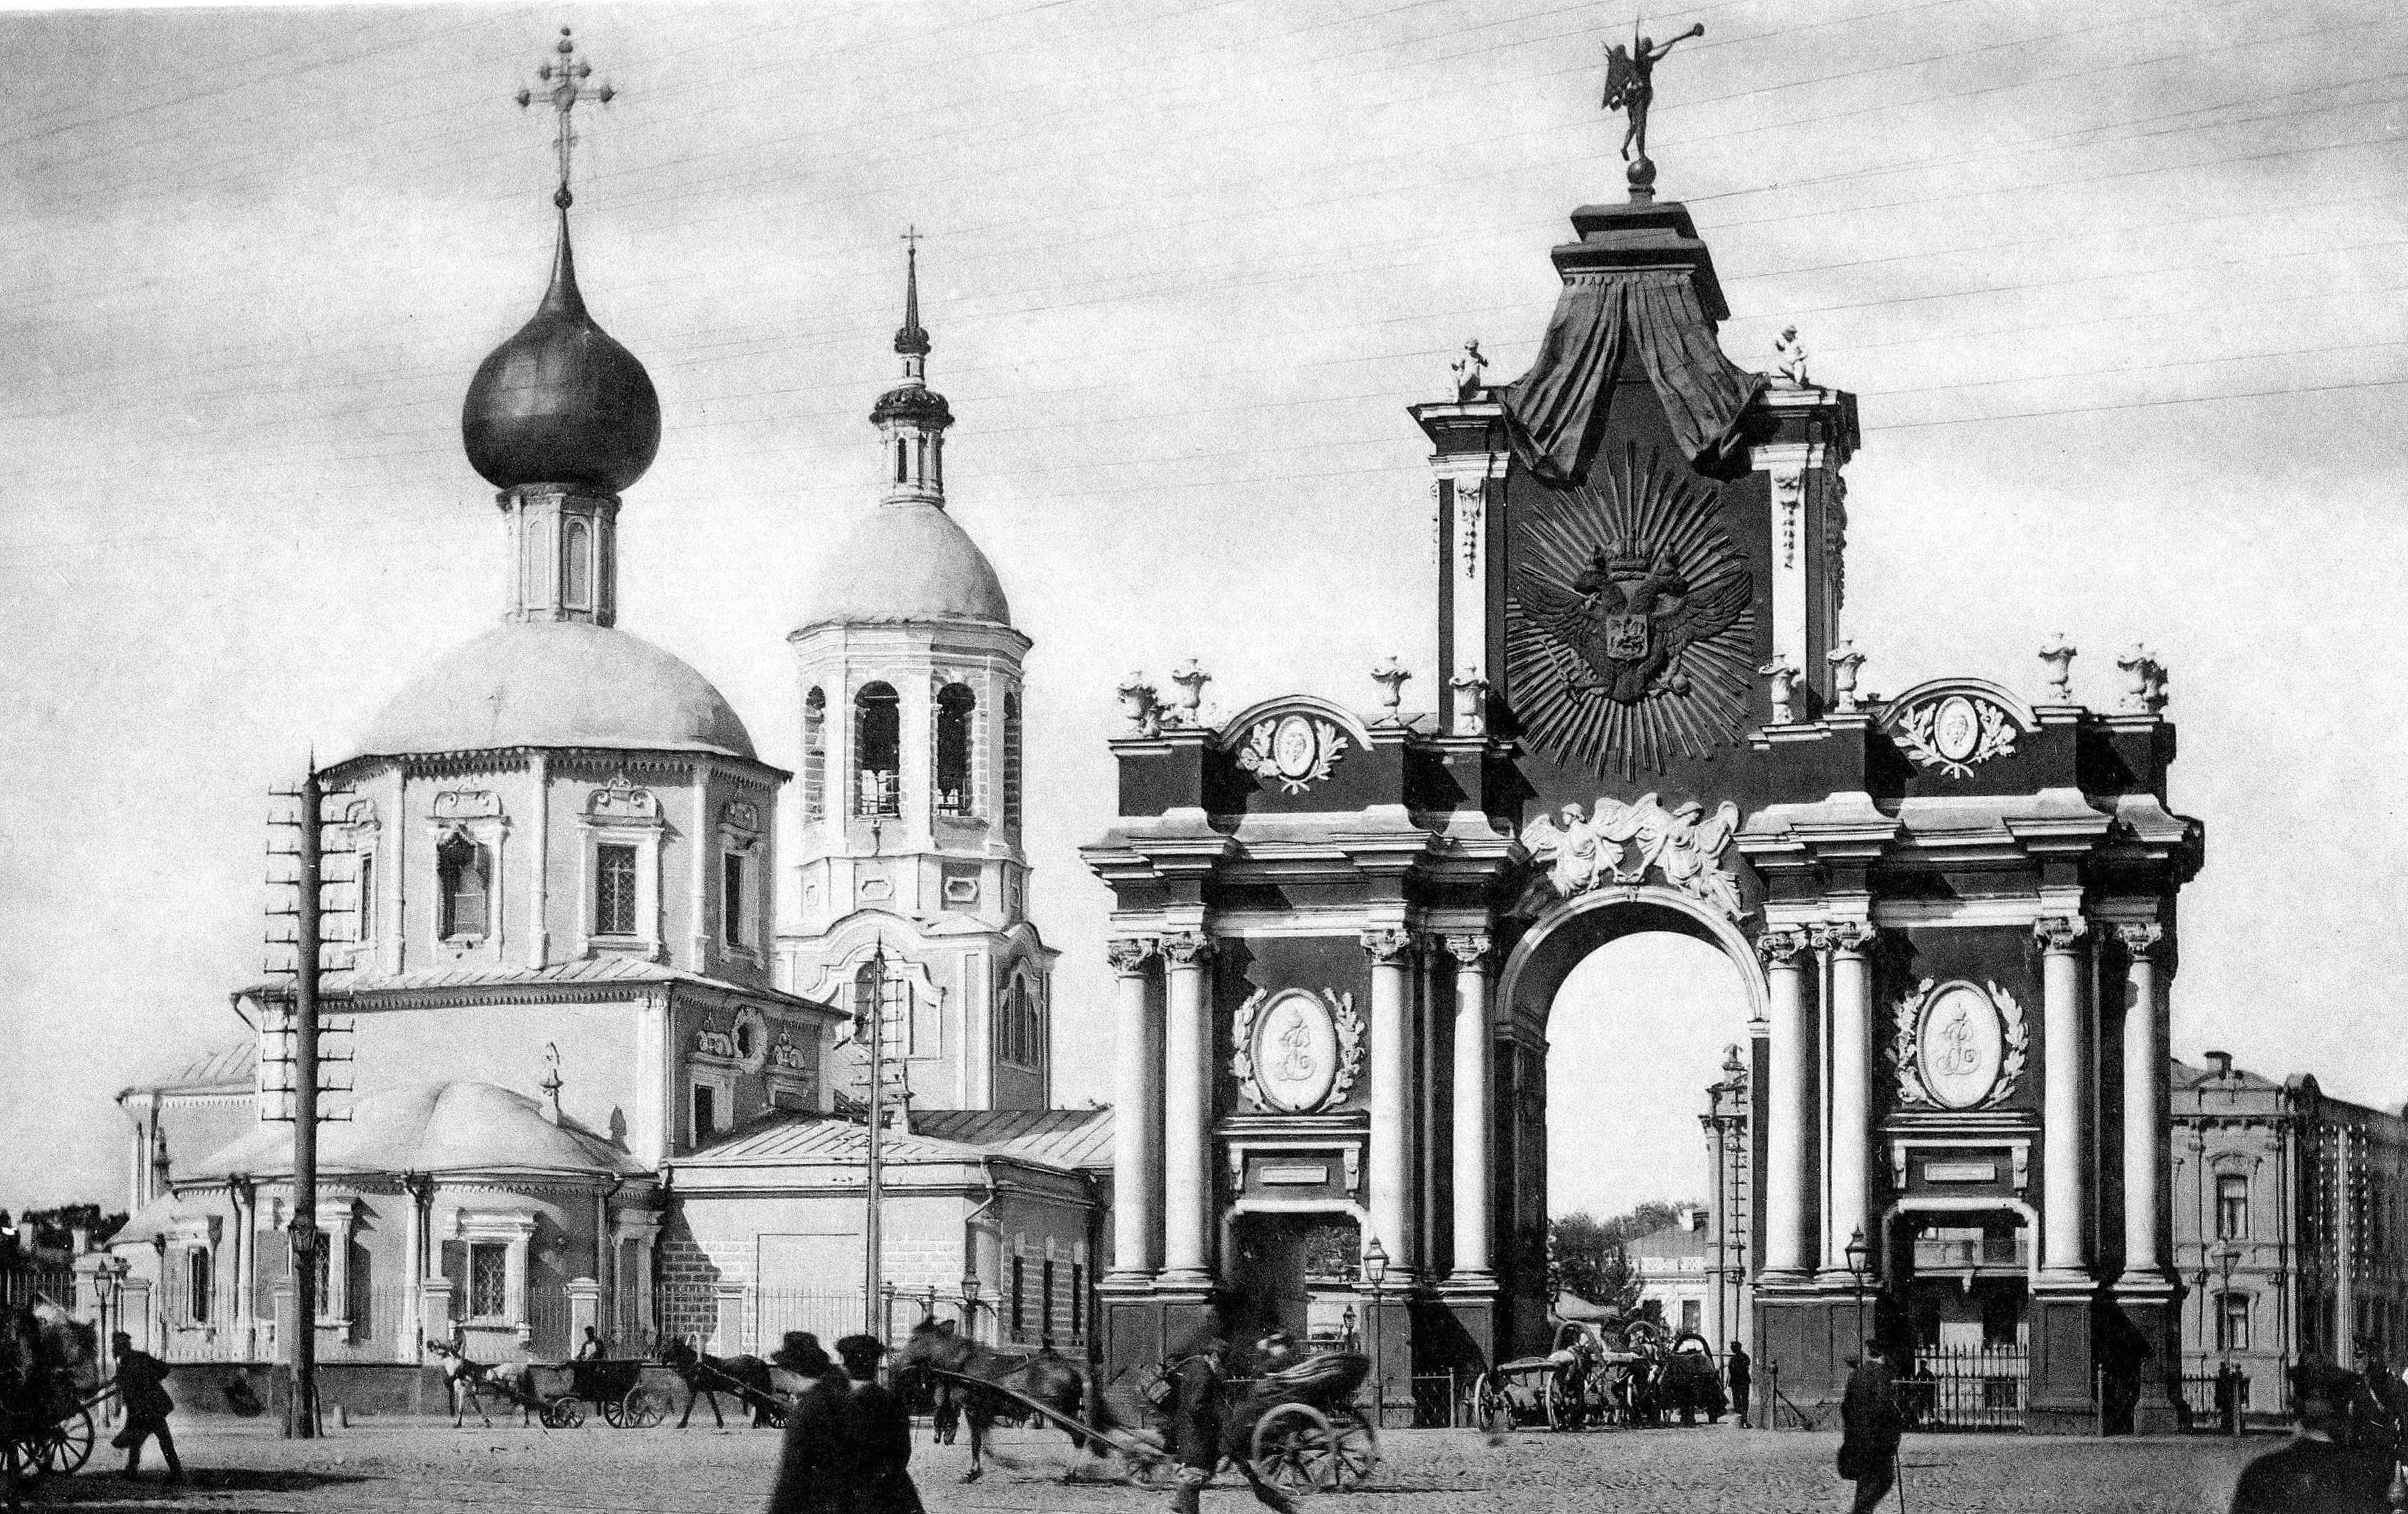
\includegraphics[width=.52\paperwidth]{inc/Title.jpg}
\end{figure}

\vfill

2012

\end{center}

\newpage

\thispagestyle{empty} 


\newgeometry{top=5cm,left=4cm,right=35mm}


\textit{Как и все предыдущие мои книжки, эту также набрал, оформил и отпечатал сын Миникс В. М.}



\newpage
\restoregeometry


\chapter{Предисловие}

\noindent
Совет ветеранов микрорайона, куда входит дом 2/6 по Хоромному тупику~-- Дом у Красных ворот, под руководством Т. В. Меньшиковой, которая продолжает дело своего отца, ведет подготовку к выпуску памятного альбома, посвященного истории и людям этого дома.

\vspace{10pt}

\begin{figure}[ht]
  \centering
  \begin{minipage}{7cm}
  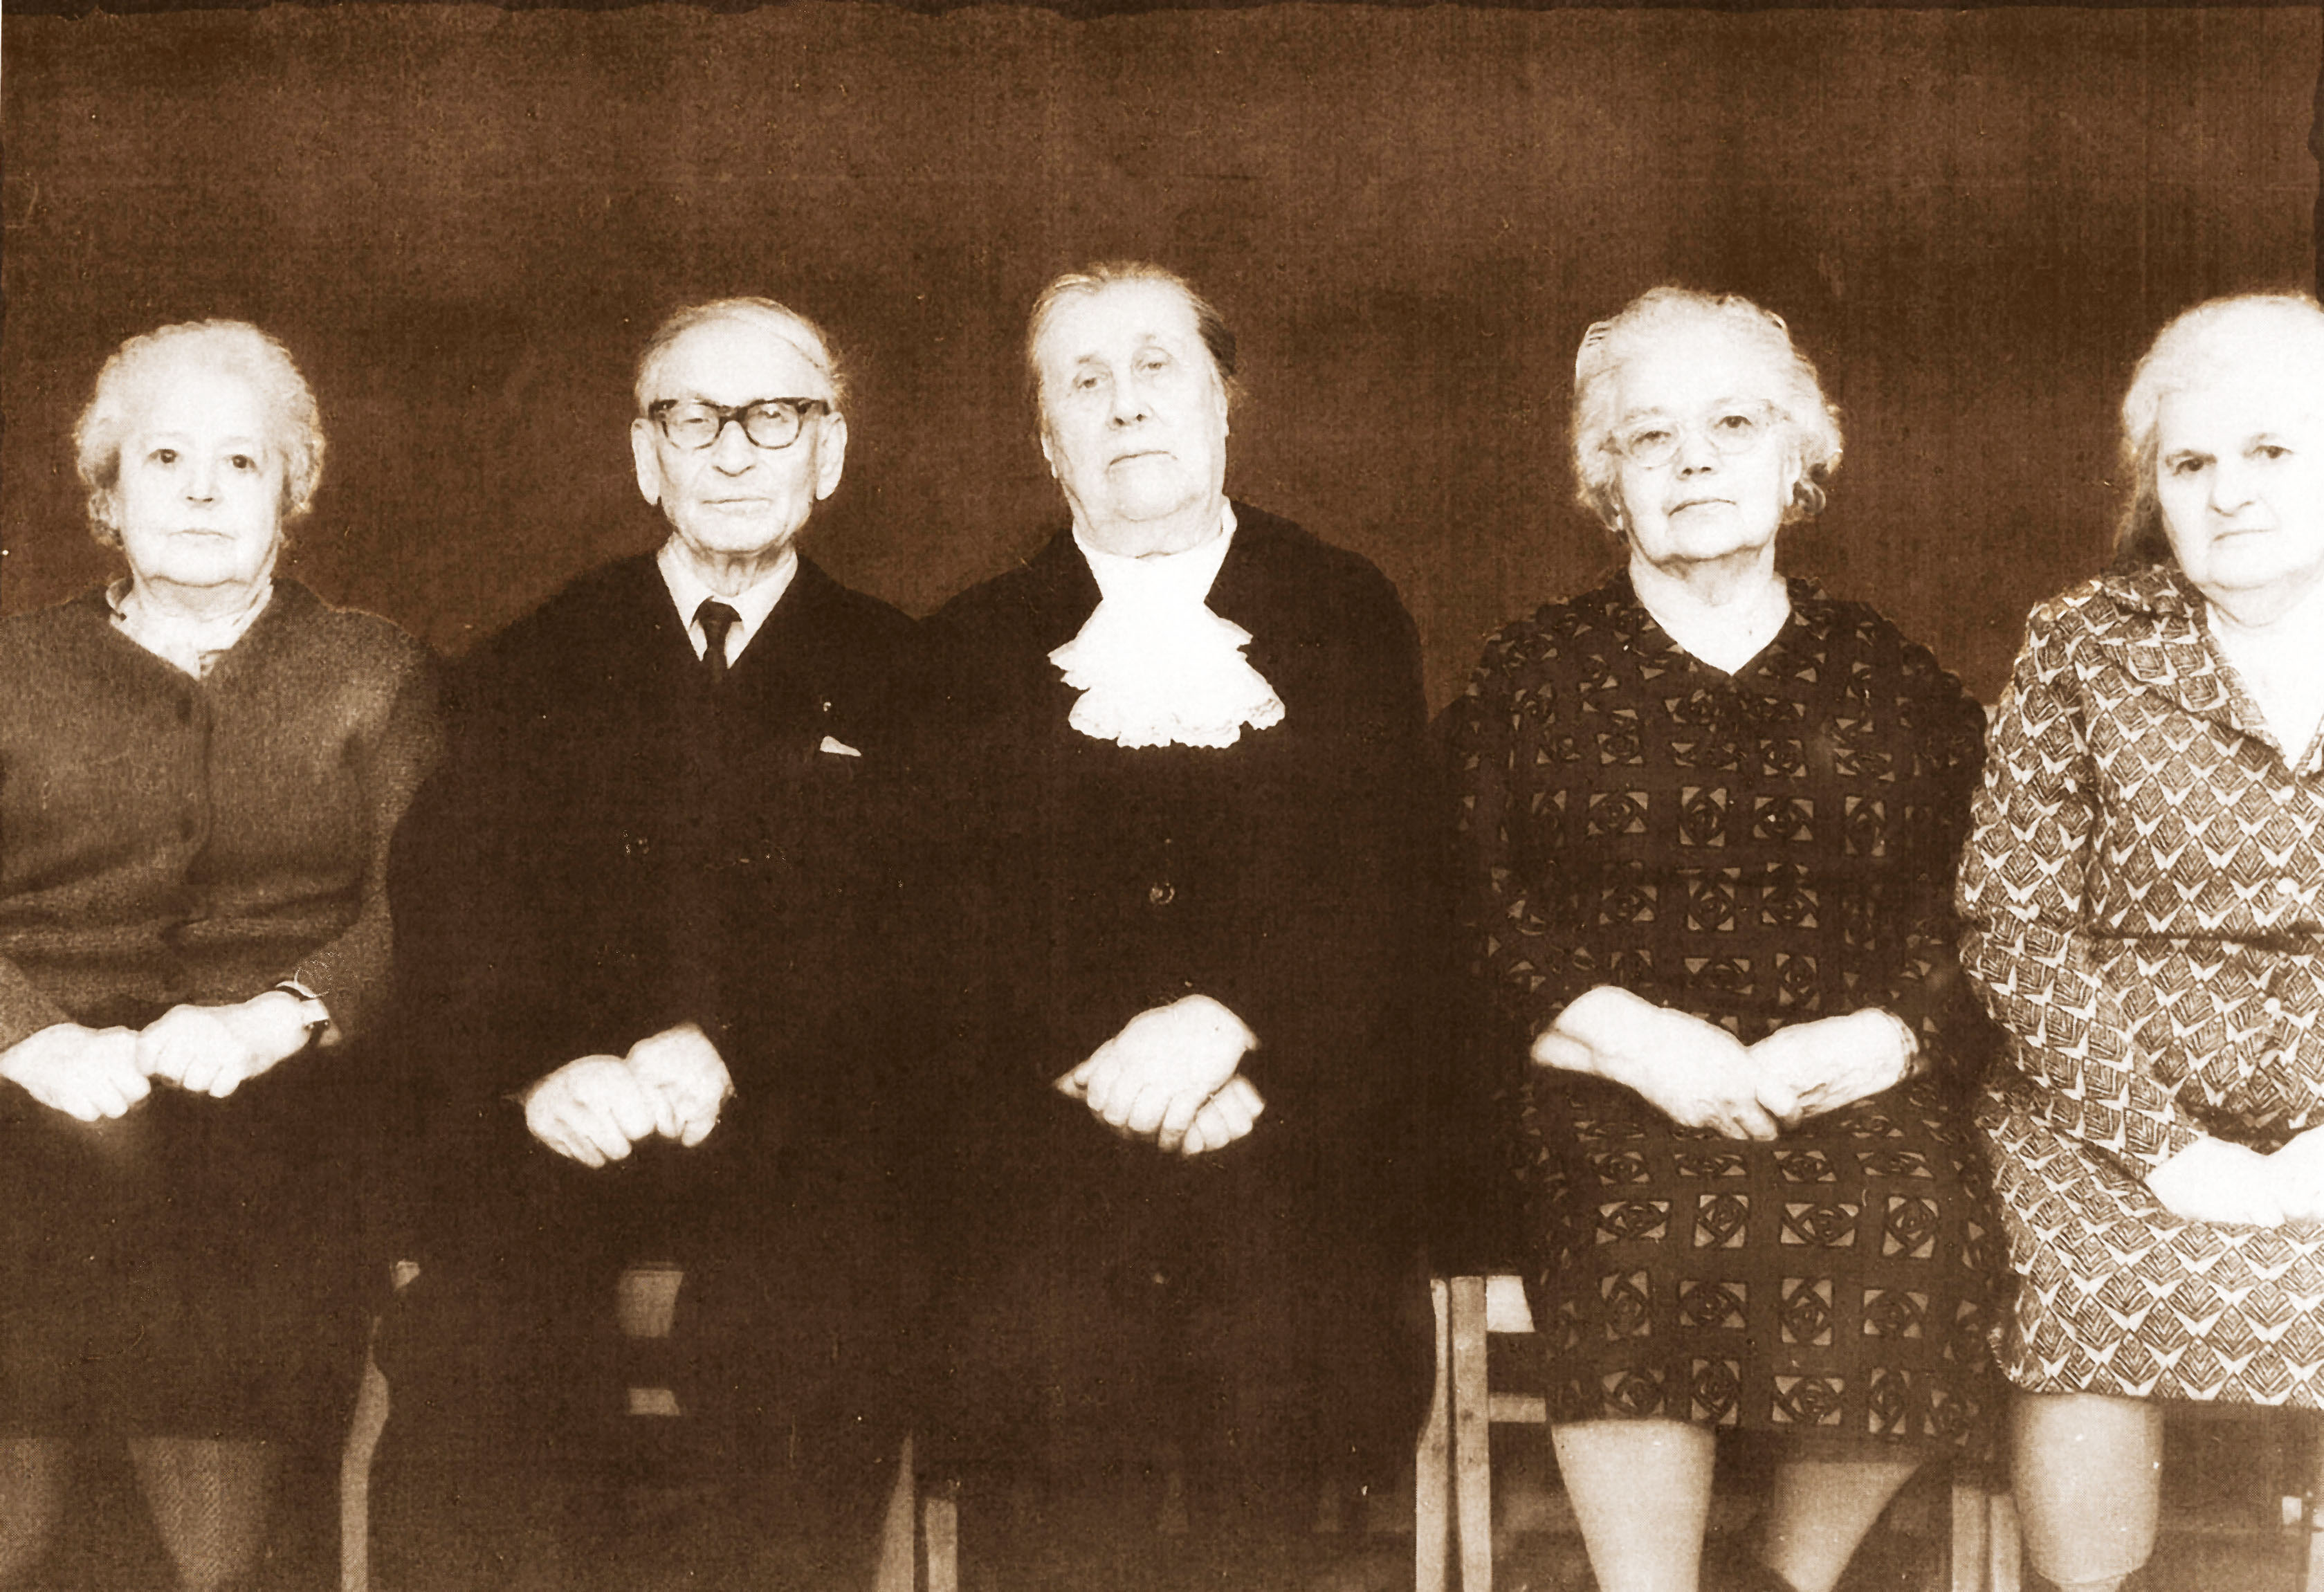
\includegraphics[width=7cm]{inc/3/1}
  \textit{\footnotesize{ Старший по Дому Меньшиков В. А. и его гвардия из <<первопоселенцев>>.}}
  \end{minipage}
\end{figure}

Предполагается, по-возможности, собрать и в систематизированном виде представить фактические данные и фотографии, в первую очередь относящиеся к <<первопоселенцам>> и семьям, въехавшим в дом в тридцатых-сороковых годах прошлого века.

Фотографии, представленные здесь, хорошо бы дополнить видом площади с <<живыми>> Красными воротами, а может быть и другими.

Вводный раздел, кроме статьи авторов-составителей Т. В. Меньшиковой и К. Д. Варзар, мне кажется, хорошо бы дополнить отрывками об истории Дома из воспоминаний ветеранов (см. Приложения).

Если удастся добраться до архивных документов~-- старых домовых книг, будет дан полный поквартирный список <<первопоселенцев>> и <<второпоселенцев>> (30-е, 40-е годы).

Совет ветеранов провел большую работу по формированию, проверке и систематизации списков репрессированных жильцов Дома, в первую очередь в 1937~-- 1939 гг., и реабилитированных (часто~-- посмертно) в 1956 г. <<за отсутствием состава преступления>>. Соответствующие списки будут опубликованы в Альбоме.

Этот Совет долгие годы занят благородным делом~-- помогает ветеранам Великой Отечественной войны, рассказывает о них, отмечает с ними торжественные события и памятные даты, что, конечно же, тоже будет отражено в Альбоме. Особая страница будет посвящена погибшим на этой войне. Не будут забыты и герои тыла.

Хорошо было бы по самостоятельной странице посвятить жильцам~-- семьям каждой из 97 квартир Дома. Но, к сожалению, через столько десятилетий раздобыть исчерпывающие данные, а особенно фото, невозможно.
Поэтому придется опубликовать только то, что удастся собрать. 

Ниже для примера в алфавитном порядке приведены данные\footnote{В Альбоме такие композиции будут размером 20 на 30 см.} о шести семьях: Варзаров, Кузнецовых, Меньшиковых, Миниксов, Моргуновых и Плоткиных.


\newgeometry{left=0mm, right=0mm, top=0mm, bottom=0mm}

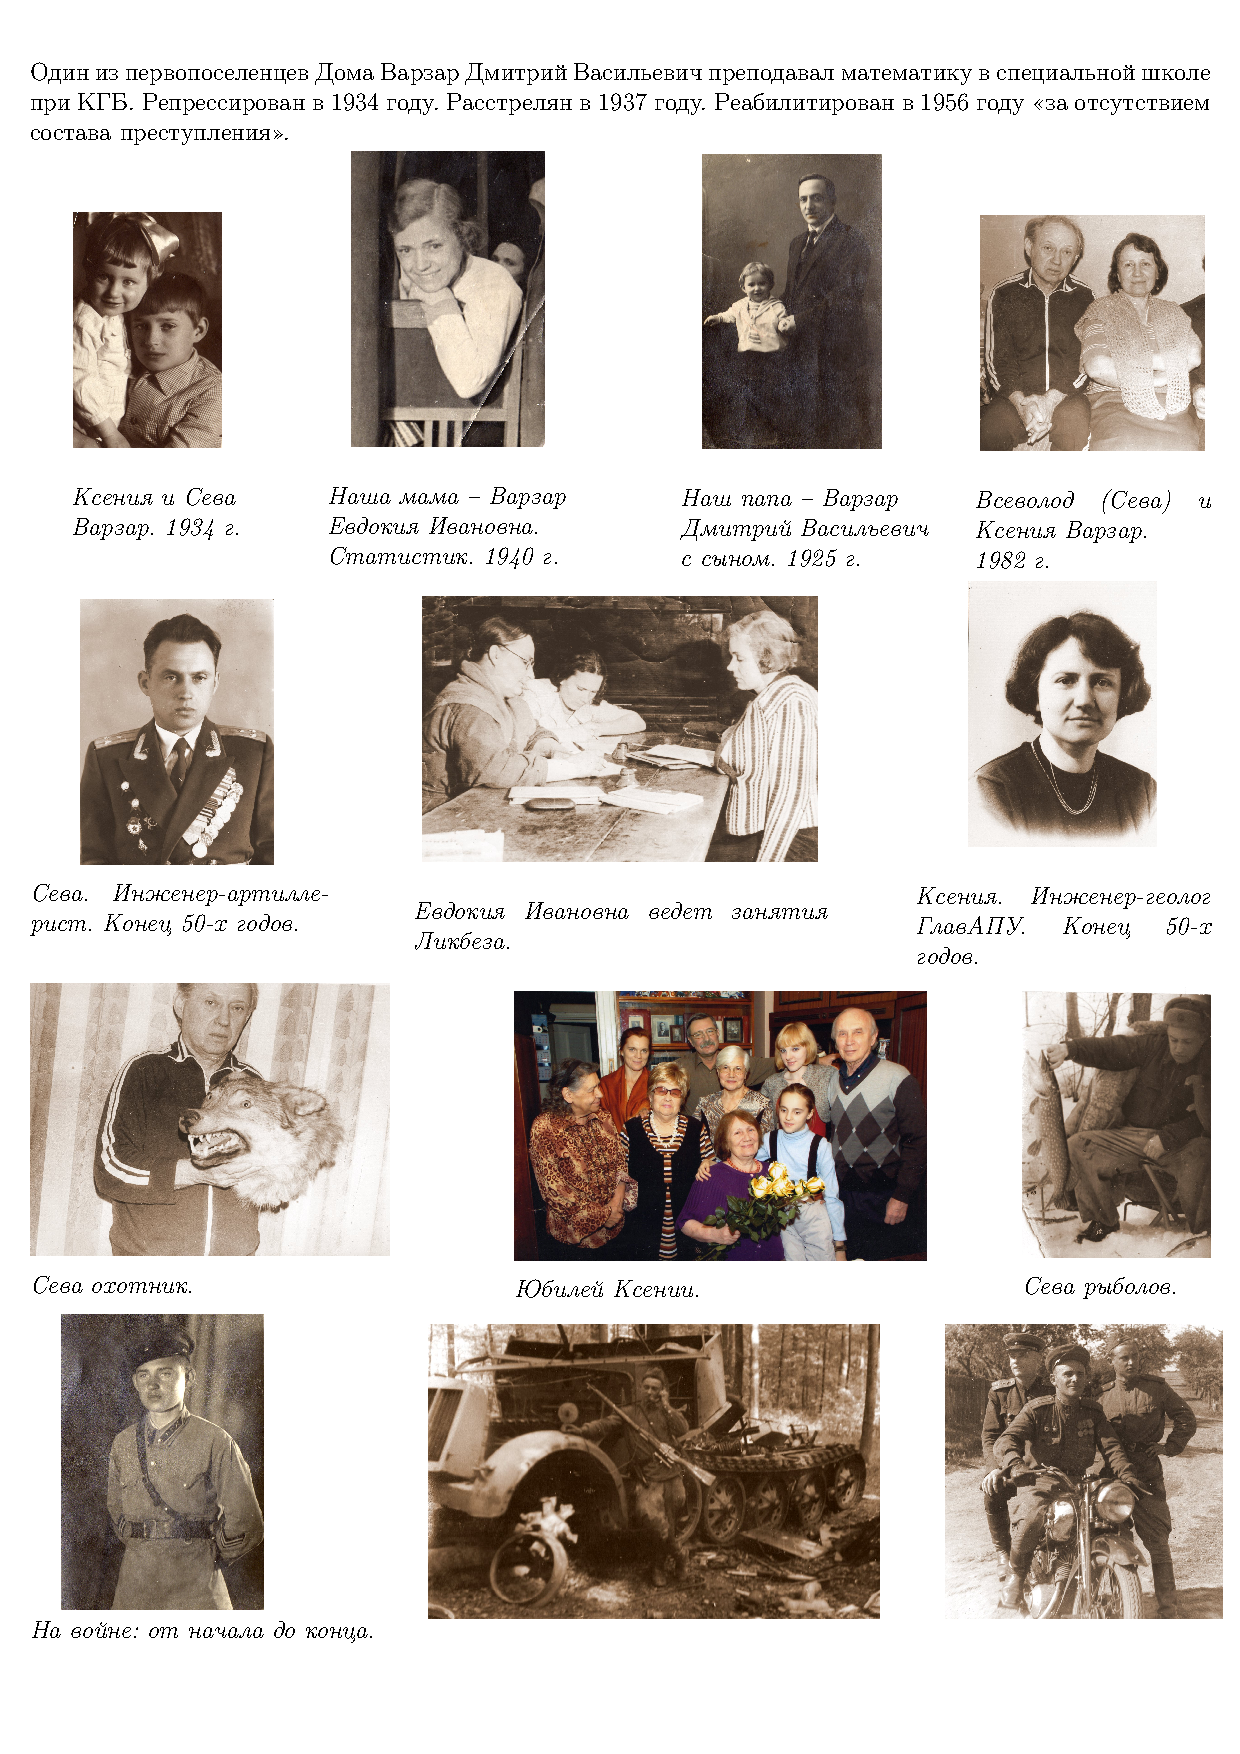
\includepdf[pages=-]{inc/varzar.pdf}

\noindent
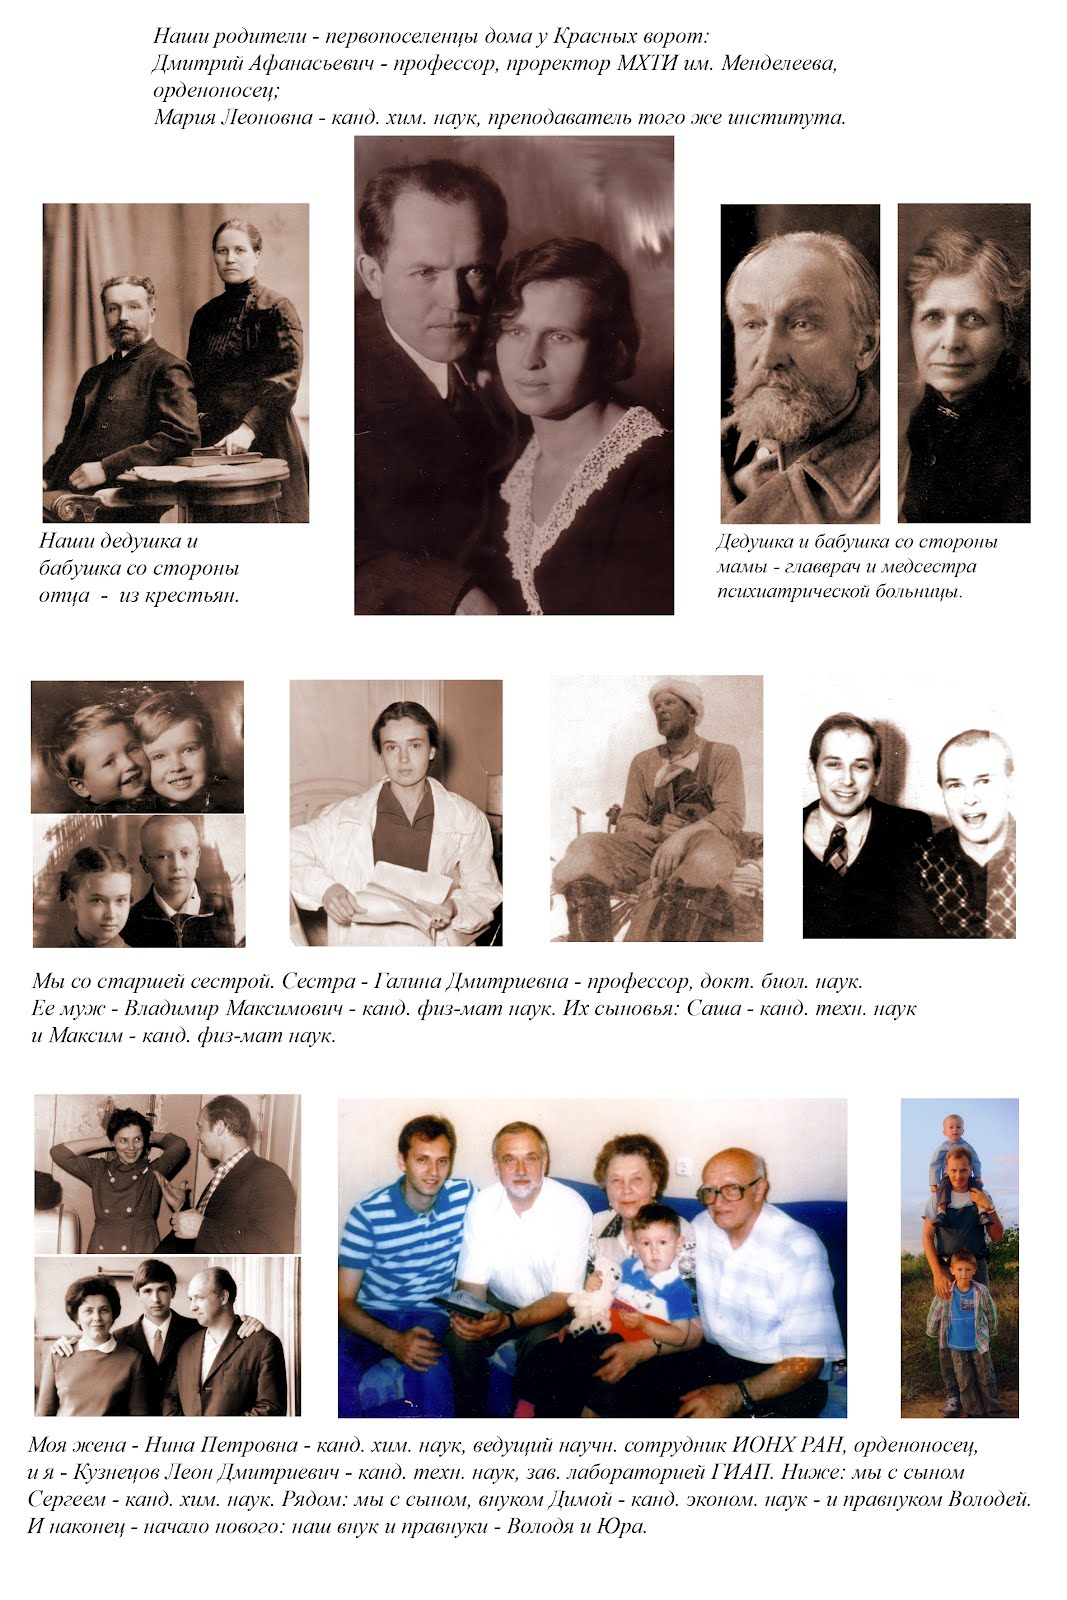
\includegraphics[height=\paperheight]{inc/kuznecovy}


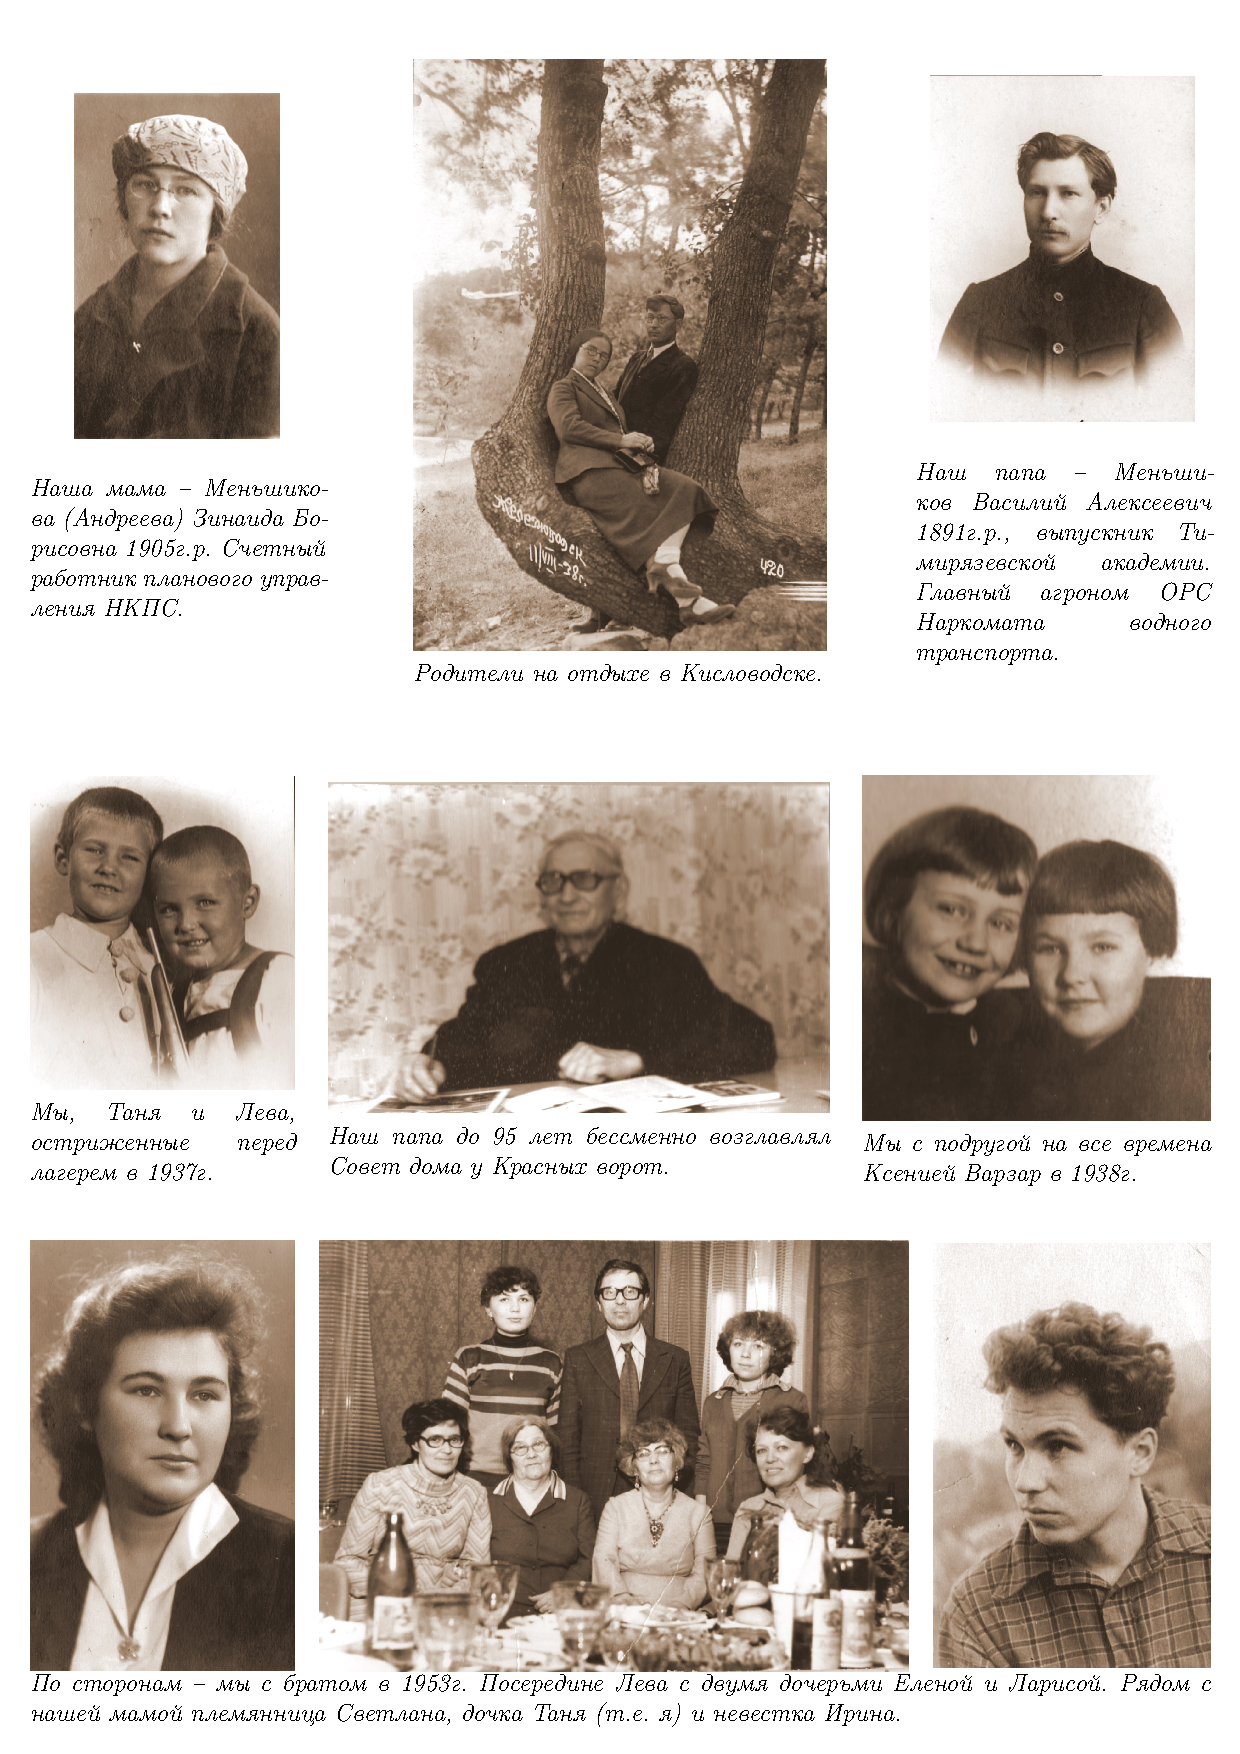
\includepdf[pages=-]{inc/menshekovy.pdf}


\begin{center}

\noindent
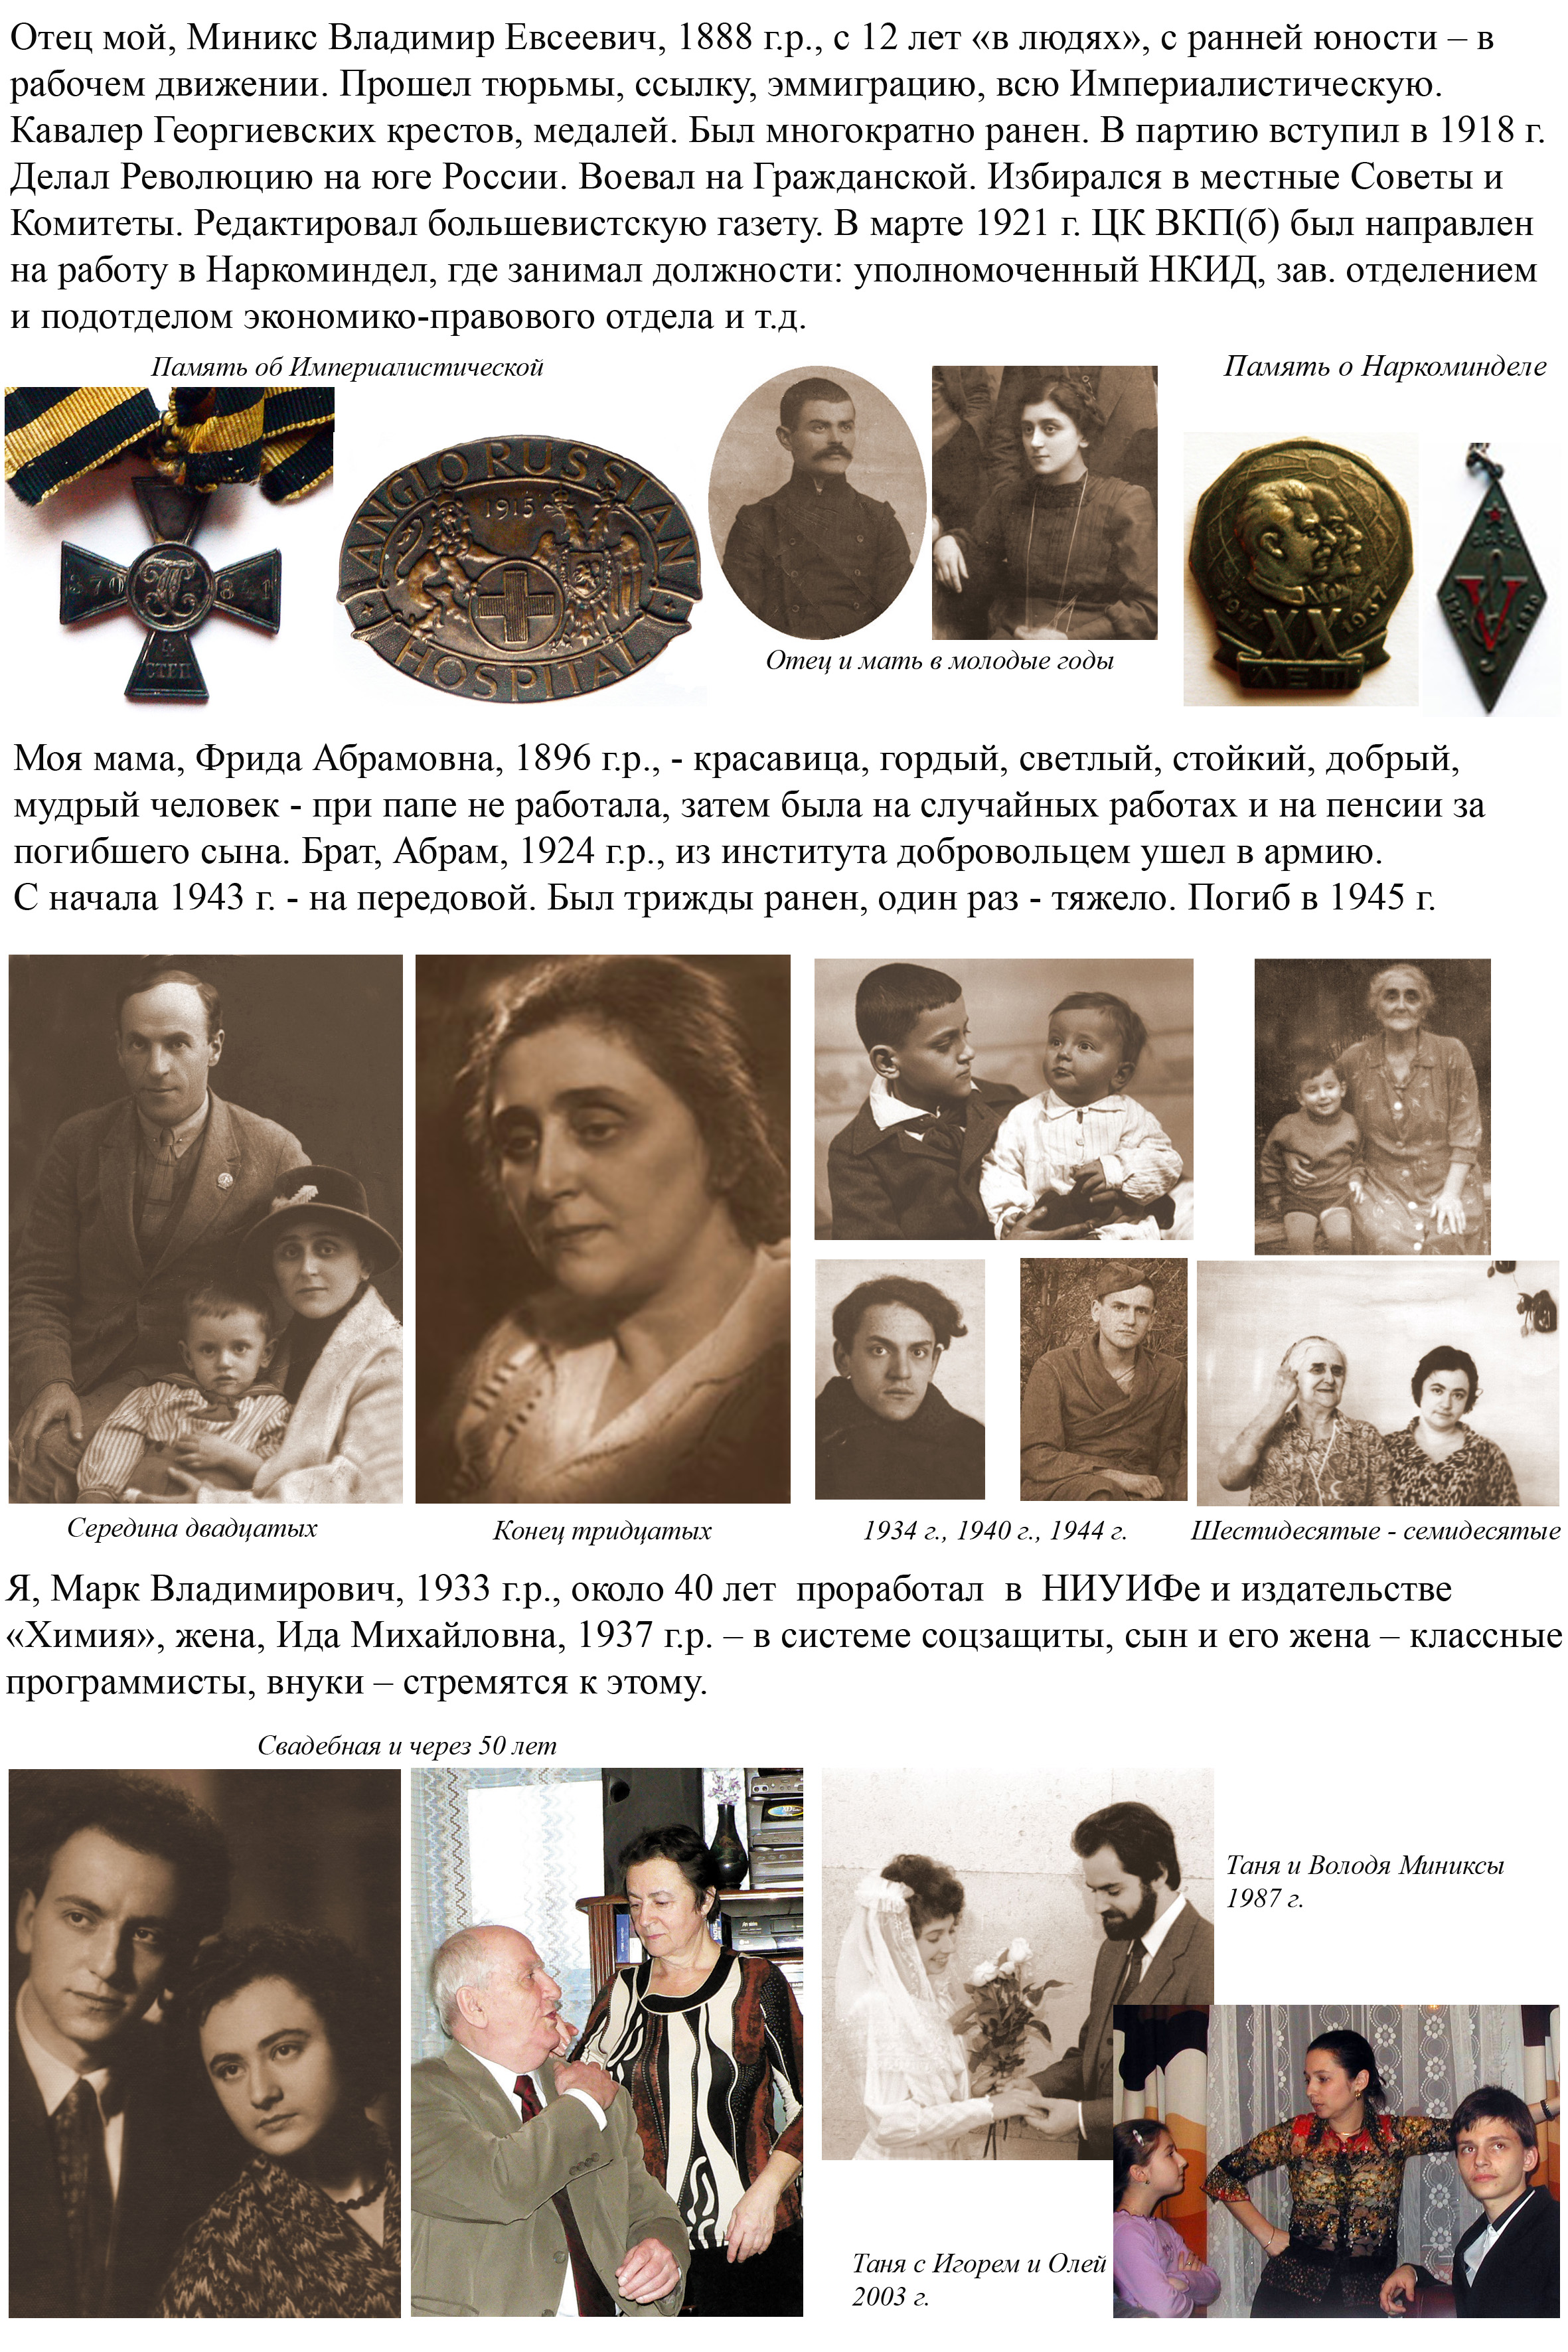
\includegraphics[height=\paperheight]{inc/minixy}

\noindent

\includegraphics[height=\paperheight]{inc/morgunovy}

\noindent
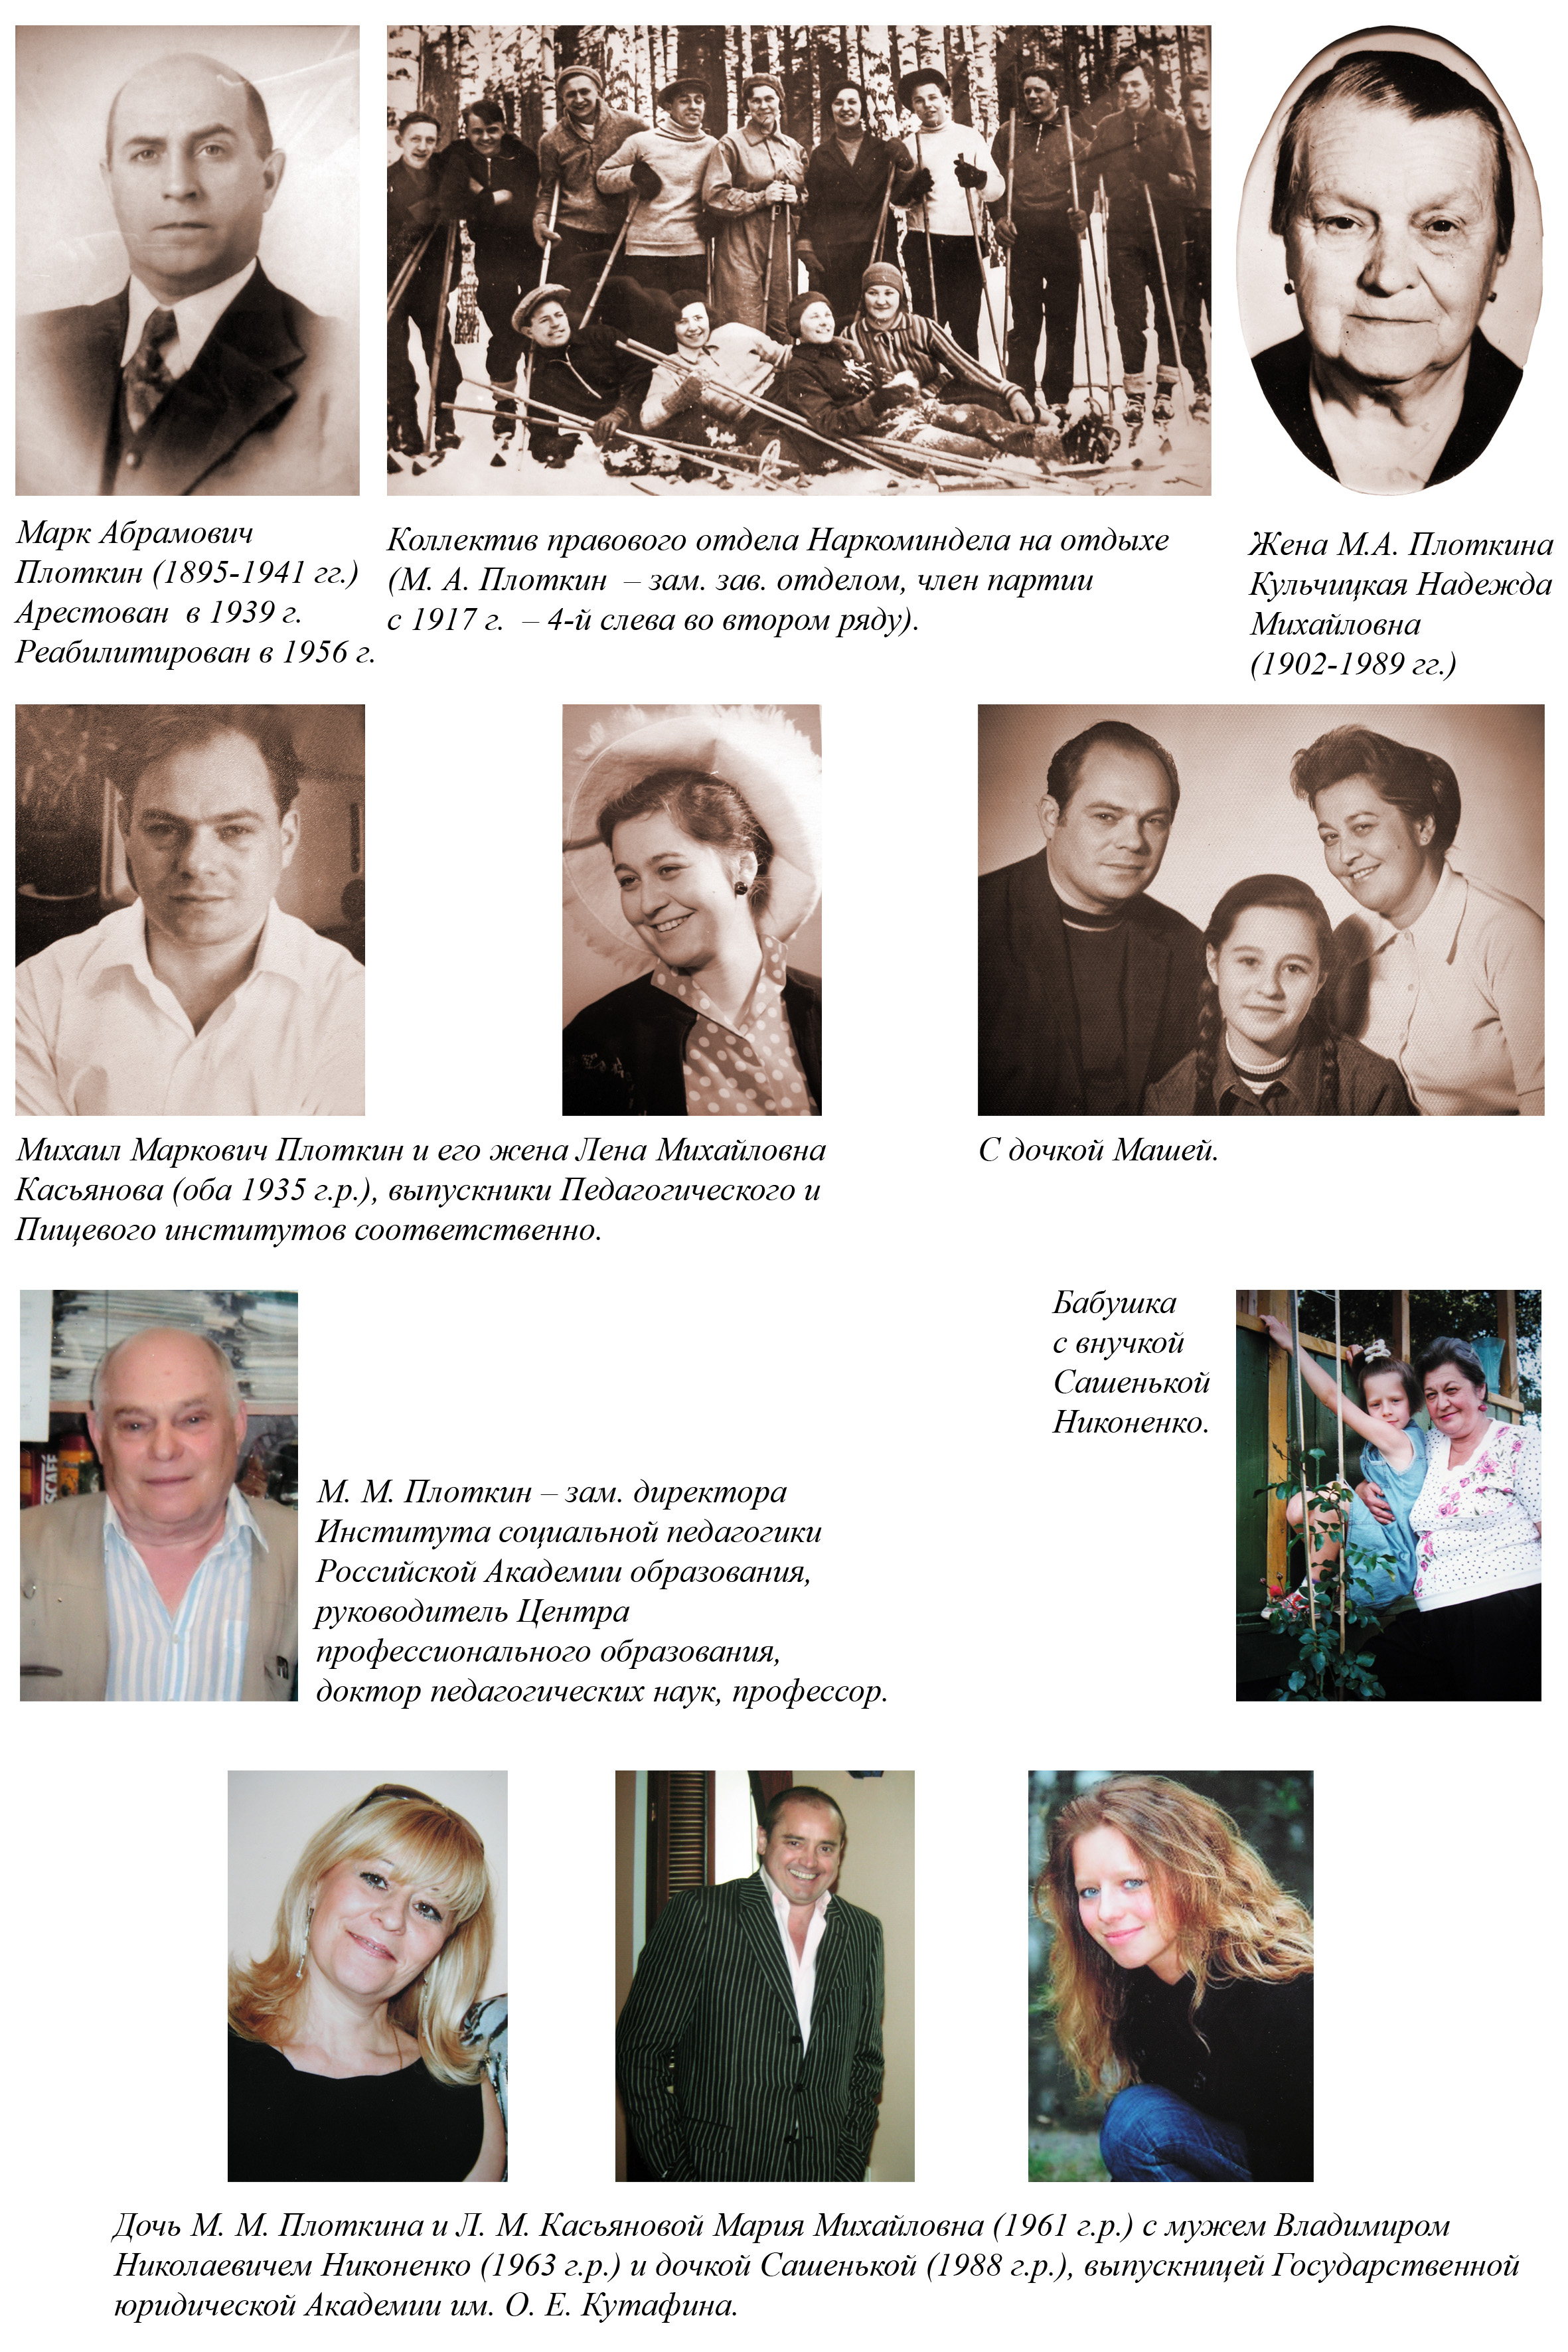
\includegraphics[height=\paperheight]{inc/plotkiny}

\end{center}

\restoregeometry



\chapter{Дворовые компании}

Многие данные и фоотографии предоставлены мне Т. В. Меньшиковой. Ей же благодарен за добрые советы.

Мне поручили написать о дворовых компанях, что я и постараюсь сделать с учетом <<собирательных>> свойств нашего Дома за период с тридцатых до шестидесятых годов. Аналог этого книжного варианта, естественно, будет в Альбоме.

Нельзя не сказать, что среди первопоселенцев нашего дома было очень много замечательных людей, начиная с Народного Комиссара иностранных дел М. М. Литвинова, его заместителей, руководителей подразделений, Чрезвычайных и полномочных посло того времени.

Сейчас, через 80 с лишним лет после заселения нашего дома, трудно сказать насколько были дружны между собой первопоселенцы, были ли дворовые компании у их старших детей (до 1920 года рождения), привлекались ли в эти компании ребята из других домов, что было характерно для последующих поколений, когда компании формировались из ребят окрестных дворов, как правило, в возрастном диапазоне 2-3 года с вкраплениями до 5 лет.

Собирательная особенность нашего двора наметилась еще до Войны, у ребят около 1924 года рождения, в основном выпускников школ 1941 года. К ним относятся: Бабенко И. Я., Багун Ю. (воевал), Варзар Сева (прошел всю войну), Дивильковский Юра (погиб), Клейн Наташа (воевала), Короткин Жора (погиб), Кунина Ляля (воевала), миникс Аба (погиб).

\newpage % ??
\newgeometry{left=10mm, right=10mm, top=5mm, bottom=0mm}

\begin{center}
    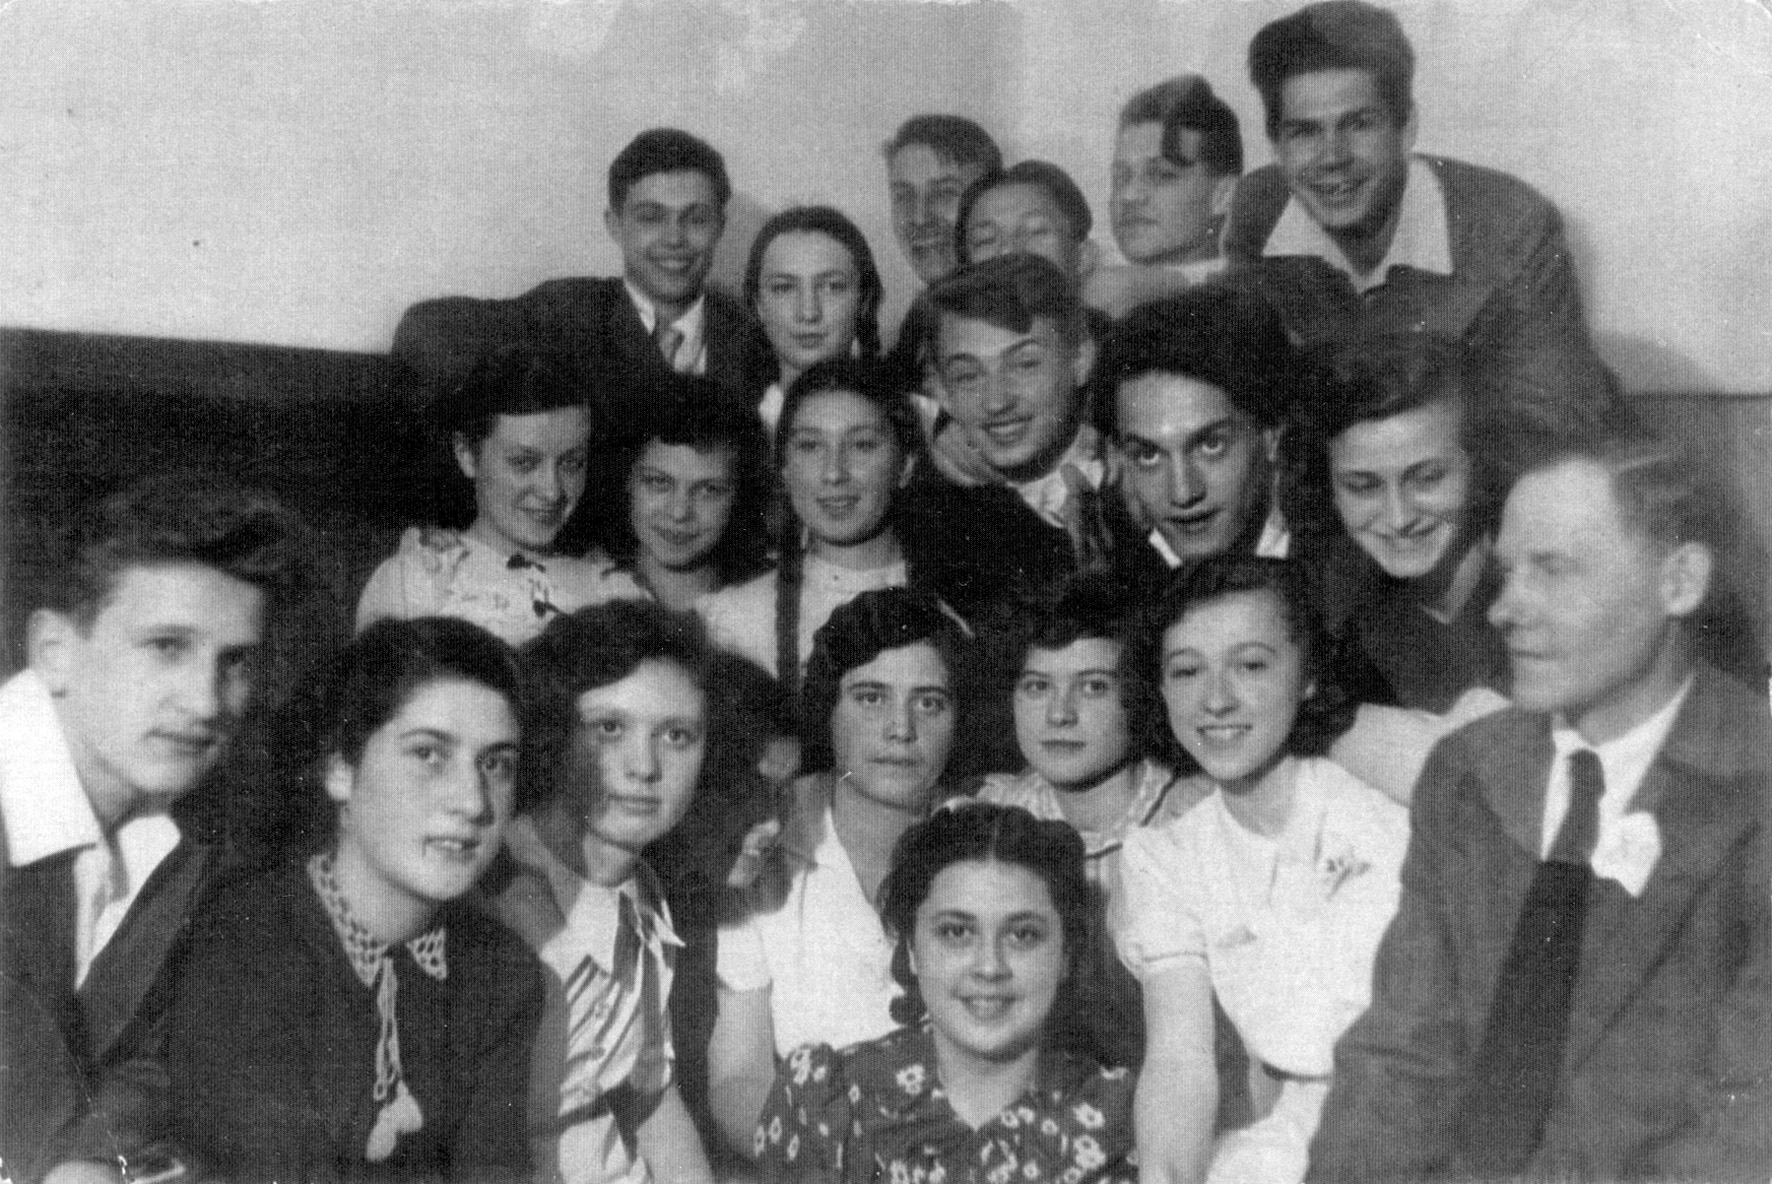
\includegraphics[width=0.5\textwidth]{inc/MalDev}
\end{center}
\begin{center}
    \footnotesize{
    \textbf {Мальчикам и девочкам 1940-х} \\
    (1924 года рождения)
    }
\end{center}

\scriptsize{
\begin{multicols}{2}
    
    \noindent
    К ребятам нашего двора \\
    Пришла не лучшая пора. \\
    \vfill
    \noindent
    Груз годов ведь с плеч не скинешь,\\
    И, куда не поглядишь,\\
    Всюду виден, вроде, фииниш,\\
    И осталось, вроде, шиш! \\
    \vfill
    \noindent
    Только нам, знать, срок не вышел,\\
    Только порох, видно, есть,\\
    Коли вновь мы, братцы, здесь,\\
    Коль мы снова тут, под крышей\\
    Дома номер два дробь шесть.\\
    \vfill
    \noindent
    Откуда шли, шпана дворовая,\\
    Когда пришла пора суровая\\
    Расстаться, шумною толпой\\
    В жизнь, как на праздник~--пей да пой!,--\\
    Ушли веселую шурьбой.\\
    Да каждый со своей судьбой.\\
    \vfill
    \noindent
    Пошли, в цепочку растянувшись,\\
    Один, едва начав, споткнувшись,\\
    Далече не успел уйти\\
    По незавдному пути;\\
    Другой, гляди, взлетел высоко,\\
    А третий ускакал далеко...\\
    \vfill   
    \noindent 
    А мир для всех куда как шире;\\
    В иных домах на нашец жизни ткань:\\
    То~-- шелк с парчей, то~-- просто дрянь!\\
    То планов дрезких грамадье,\\
    То только старое тряпье.\\
    \vfill
    \noindent
    Но жизнь~-- от Бога и надолго.\\
    И не забыть бы, братцы, долга\\
    За нами~-- тем, кто нас родил,\\
    Да тем, кто раньше уходил.\\
    Но не в прекрасную страну,\\
    А на проклятую войну.\\
    \vfill
    \noindent
    Утащила злая баба,\\
    Уложила в поле сдуру\\
    Твоео братишку Абу,\\
    Моего братана Юру,\\
    Сколько было их~-- не счесть!\\
    Всех помянем благородно,\\
    Отдадим посмертно честь!\\
    \vfill
    \noindent
    С непкурытой головою,\\
    То ли лысой, то ль седою,\\
    Постоим да помолчим.\\
    А потом уж прокричим\\
    Из последних сил, что есть,\\
    Славу дому два дробь шесть!\\
\end{multicols}
\vspace*{-5mm}
\raggedleft{С. И. Д. (Дивильковский С. И.), 2010 г.

}
}


\restoregeometry

\mainmatter % это включает нумерацию глав и секций в документе ниже



\backmatter %% Здесь заканчивается нумерованная часть документа и начинаются ссылки и
            %% заключение



\appendix   % Тут идут приложения



\end{document}

%%% Local Variables:
%%% mode: latex
%%% TeX-master: t
%%% End:
